\clearpage
\section{Learning curves and first-update erosion}\label{app:curves}
% Built from ledger-bound values; edit the script, not this table.
\begingroup\fontsize{8}{9.5}\selectfont\setlength{\tabcolsep}{3pt}\emergencystretch=1em\hyphenpenalty=10000\exhyphenpenalty=10000
\begin{longtable}{@{}>{\raggedright\arraybackslash}p{1.967in}>{\raggedright\arraybackslash}p{1.967in}>{\raggedright\arraybackslash}p{1.967in}@{}}
\caption{Analytical appendix D. Exact recorded counts or decisions; no pooled reader accuracies. Complete support, settings, controls and per-seed records are in the numbered supplementary tables and released data.}\label{tab:compact_D}\\
\toprule
\textbf{update-1 condition} & \textbf{correct counts (seeds 0/\allowbreak{}1/\allowbreak{}2)} & \textbf{histories per seed} \\
\midrule\endfirsthead
\toprule
\textbf{update-1 condition} & \textbf{correct counts (seeds 0/\allowbreak{}1/\allowbreak{}2)} & \textbf{histories per seed} \\
\midrule\endhead
\midrule\multicolumn{3}{r}{Continued on next page}\\\endfoot
\bottomrule\endlastfoot
AdamW & 393 /\allowbreak{} 5 /\allowbreak{} 518 & 1,555 \\
reduced-lr AdamW & 1554 /\allowbreak{} 1468 /\allowbreak{} 1553 & 1,555 \\*
SGD & 1440 /\allowbreak{} 89 /\allowbreak{} 1495 & 1,555 \\*
blocked prediction gradient & 1555 /\allowbreak{} 1555 /\allowbreak{} 1555 & 1,555 \\
\end{longtable}
\endgroup

All per-update local counts and movements are in Supplement Table S27.
The supplement also contains every study's learning curves, without checkpoint
selection. The figures below show why low natural KL is not a sufficient reliability
measurement, and the erosion of the sums computation against cumulative
movement.
\begin{figure}[tb]
\centering
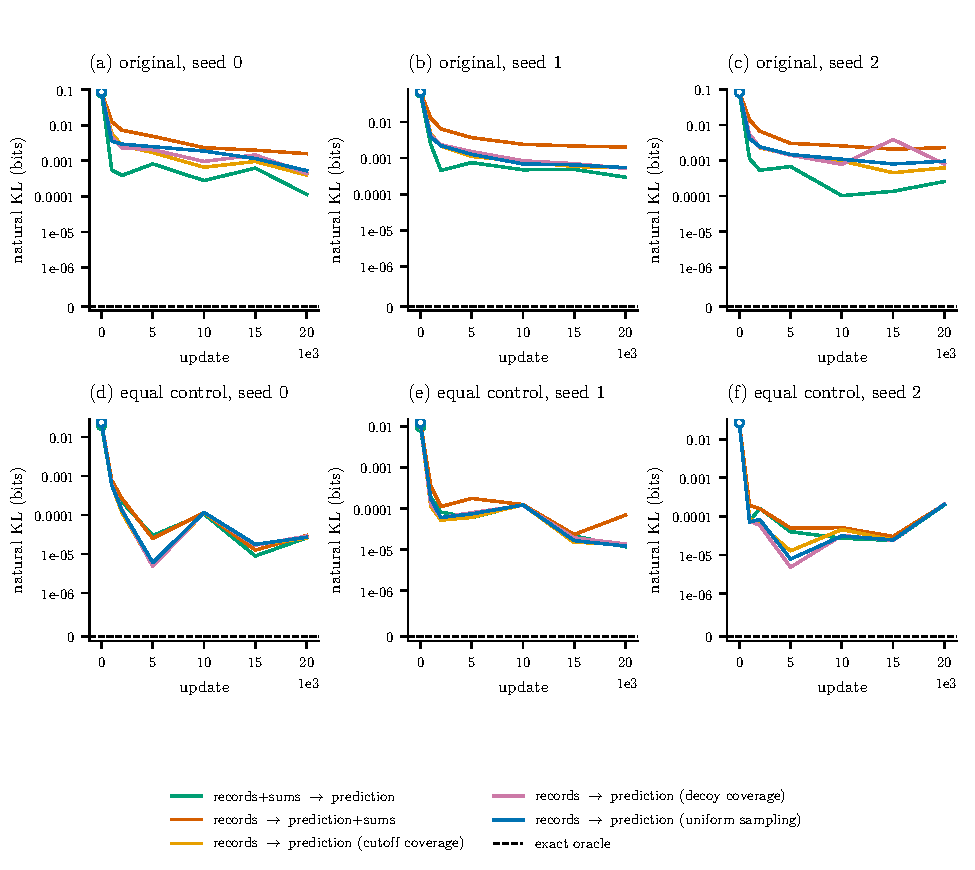
\includegraphics[width=\textwidth]{figures/appendix_D_r12.pdf}
\caption{\csname captionappendix_D_r12\endcsname}\label{fig:appendix_D_r12}
\end{figure}

\begin{figure}[tb]
\centering
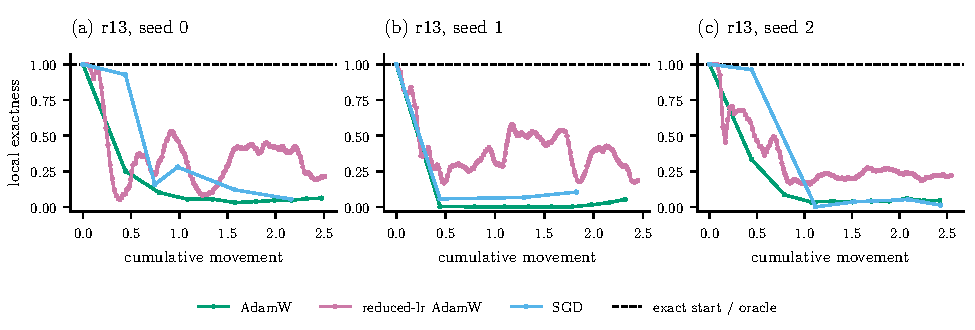
\includegraphics[width=\textwidth]{figures/appendix_D_movement.pdf}
\caption{\csname captionappendix_D_movement\endcsname}\label{fig:appendix_D_movement}
\end{figure}

\begin{figure}[tb]
\centering
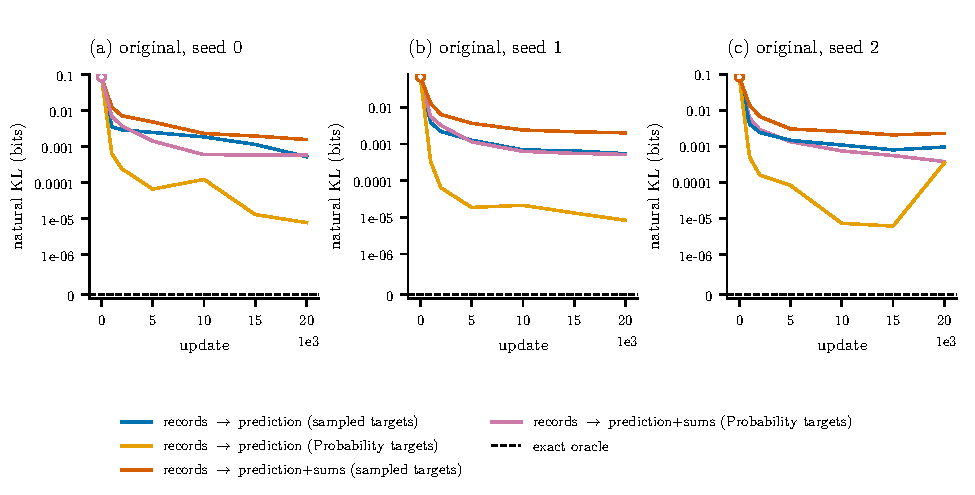
\includegraphics[width=\textwidth]{figures/appendix_D_r13_noise.pdf}
\caption{\csname captionappendix_D_r13_noise\endcsname}\label{fig:appendix_D_r13_noise}
\end{figure}

